\documentclass[xcolor=pdftex,dvipsnames,table,mathserif,aspectratio=169]{beamer}
\usetheme{default}
\usetheme{metropolis}
%\usepackage{minted}
\usepackage{mathtools}
\setbeamersize{text margin left=.3in,text margin right=.3in} 

\usepackage[english]{babel}
\usepackage{pgf,pgfarrows,pgfnodes,pgfautomata,pgfheaps}
\usepackage{amsmath,amssymb,setspace,centernot}
\usepackage[latin1]{inputenc}
\usepackage{pgf,tikz}
\usepackage[T1]{fontenc}
\usepackage{relsize}
\usepackage{pdfpages}
\usepackage[absolute,overlay]{textpos} 


\DeclareMathOperator*{\argmax}{arg\,max}
\DeclareMathOperator*{\argmin}{arg\,min}

\newcommand{\X}{\mathtt{X}}
\newcommand{\Y}{\mathtt{Y}}

%\newcommand{\R}{\mathbb{R}}
%\newcommand{\E}{\mathbb{E}}
%\newcommand{\V}{\mathbb{V}}
\newcommand{\p}{\mathbb{P}}
\newcommand*\df{\mathop{}\!\mathrm{d}}
\newcommand{\del}{\partial}


% imports
\usepackage{xargs}
\usepackage{xpatch}
\usepackage{etoolbox}
\usepackage{pdflscape}
\usepackage{booktabs}
\usepackage{threeparttable}
\usepackage[skip=0.2\baselineskip]{caption}

% command for inputting raw latex
\makeatletter
\newcommand\primitiveinput[1]{\@@input #1 }
\makeatother

% common table command
\newcommandx{\tablecontent}[4]{
    \begin{threeparttable}[!ht]
        \centering
        \caption{#3}
        \vspace{-1em}
        \footnotesize
        \begin{tabular}{#1}
            \primitiveinput{../tables/#2.tex}
        \end{tabular}
        \vspace{-0.2em}
        \begin{tablenotes}[flushleft]
            #4
        \end{tablenotes}
    \end{threeparttable}
}




% \usepackage{slashbox}
\title{ Empirical Bayes/ Shrinkage}
\author{Chris Conlon }
\institute{NYU Stern }


\newcommand{\norm}[1]{\left\lVert#1\right\rVert}
\newcommand{\R}{\mathbb{R}}
\newcommand{\E}{\mathbb{E}}
\newcommand{\V}{\mathbb{V}}
\newcommand{\ol}{\overline}
%\newcommand{\ul}{\underline}
\newcommand{\pp}{{\prime \prime}}
\newcommand{\ppp}{{\prime \prime \prime}}
\newcommand{\policy}{\gamma}


\newcommand{\fp}{\frame[plain]}

\date{\today}

\begin{document}
\maketitle
\section{Empirical Bayes}



\begin{frame}[fragile]{A (famous) Baseball Example}
Suppose we want to estimate batting averages $(AVG)$ for some baseball players
\begin{itemize}
\item $AVG = \frac{\# \text{hits}}{ \# At Bats}$
\item Use data on the first $n=45$ at bats and hits $x_i$ for the 1970 season.
\item Predict the batting average $\mu_i$ for the end of the season  ($n=400-500$ at bats).
\item Obvious estimate is batting average after 45 at bats: $\widehat{\mu}_i^{MLE}= x_i/45$.
\item Is there a better estimate?
\end{itemize}
\end{frame}


\begin{frame}[fragile]{A Baseball Example}
\begin{center}
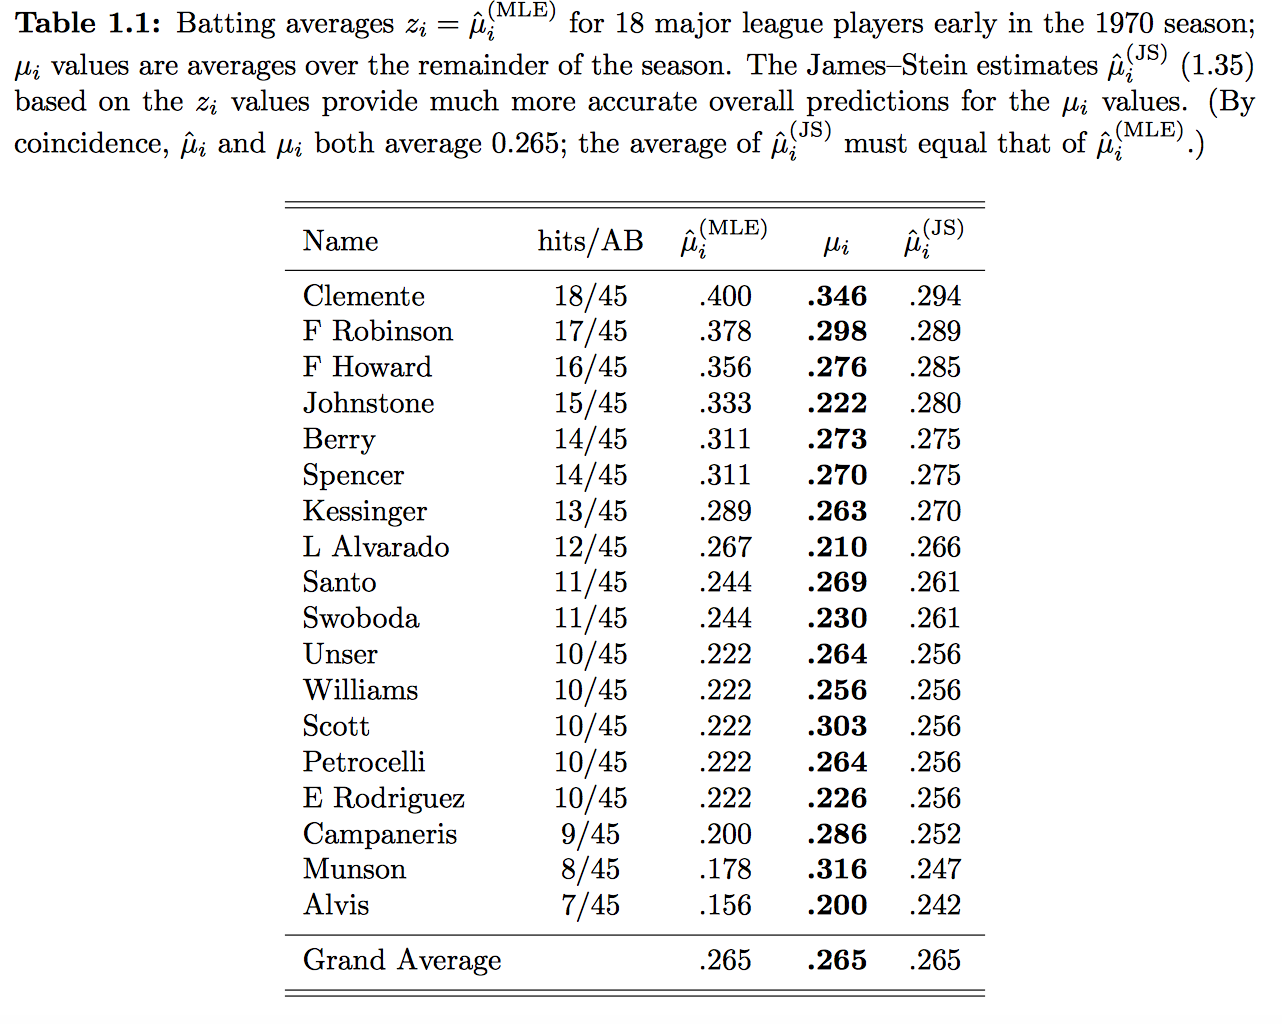
\includegraphics[width=3.5in]{./resources/baseball.png}
\end{center}
\end{frame}

\begin{frame}[fragile]{A (famous) Baseball Example}
Probably we can do better than the MLE here:
\begin{itemize}
\item Thurman Munson wins Rookie of the Year and ends up batting $\mu_i = .316$. If he batted .178 all year, his career would not have lasted long.
\item Clemente's $.400$ seems unlikely to hold up. Last player to hit $> .400$ was Ted Williams $.406$ in 1941.
\item But how?
\end{itemize}
\end{frame}

\begin{frame}[fragile]{Bayesian Shrinkage}
Idea is to take an average between the observed average $y_i$ and the overall mean $\overline{y}$:
\begin{align*}
\widehat{\mu}_i^{JS} &=  (1-\lambda) \cdot \overline{y}  + \lambda \cdot y_i, \quad
\lambda = 1 - \frac{(k-3) \sigma^2}{\sum_i( y_i - \overline{y})^2}
\end{align*}
\begin{itemize}
\item This has the effect of \alert{shrinking} $y_i$ towards the \alert{prior mean} $\overline{y}$.
\item In this case the \alert{prior mean} is just $\overline{y}$ the grand-mean of all players
\item How can information about unrelated players inform us about $\mu_i$?
\item Also consider proportion of foreign cars in Chicago as an additional $y_i$, can this help too?
\item The \alert{shrinkage factor} $\lambda$ depends on sample size and variance, but how is it chosen?
\end{itemize}
\end{frame}



\begin{frame}[fragile]{A Baseball Example}
\begin{center}
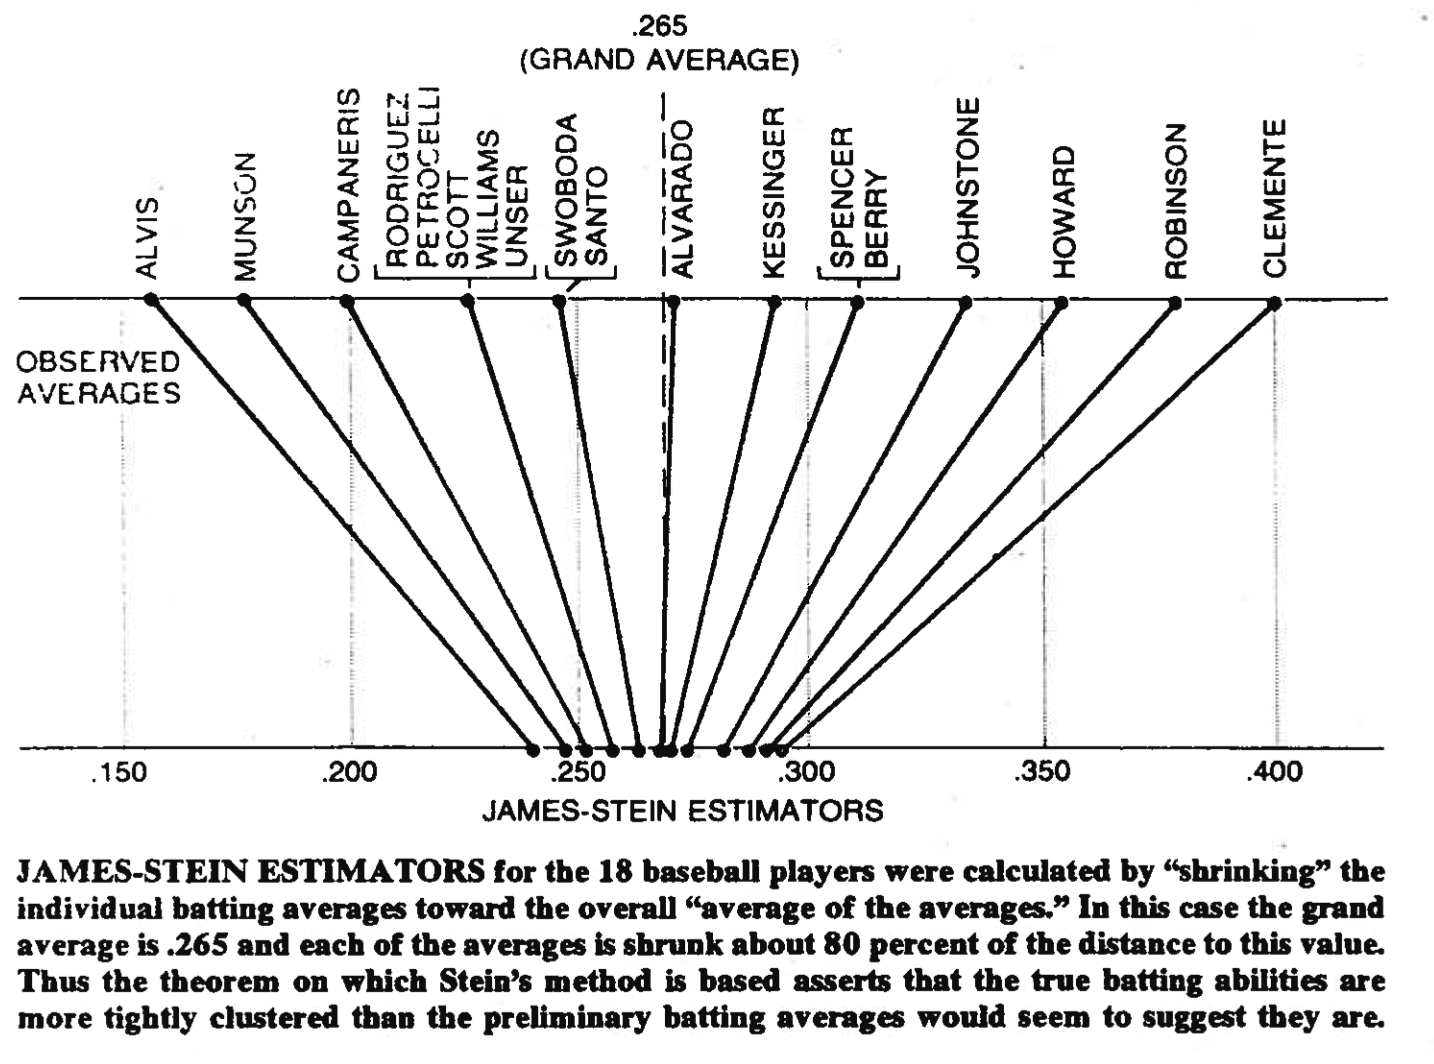
\includegraphics[width=3.5in]{./resources/baseball2.png}
\end{center}
\end{frame}

\begin{frame}{Aside: James-Stein Estimator}
This is a famous (and confusing) result from statistics:
\begin{itemize}
\item For normally distributed $Y \sim N(\theta,\sigma^2 I)$ with unknown means $[\theta_1,\theta_2,\ldots,\theta_k]$
\item Why would using information from $Y_2$ tell us anything about $Y_1$?
\item And yet the James-Stein or (pooled) shrinkage estimator is biased, but has lower MSE than the naive estimator.
\item Why does Clemente's batting average tell us anything about Munson's?
\end{itemize}
See \url{https://statweb.stanford.edu/~ckirby/brad/LSI/chapter1.pdf} for formal results.
\end{frame}

\begin{frame}{What is Emprical Bayes?}
\begin{itemize}
\item Priors can be an important modeling choice
\item But what makes a good prior?
\begin{itemize}
\item Sufficiently diffuse
\item As non-informative as possible
\item Don't tip the scales
\item Don't rule out the truth
\end{itemize}
\item Idea: can we use the data itself to construct a prior?
\begin{itemize}
\item If everything is a function of data, are we back in frequentist paradigm?
\item Can we get benefits of Bayes estimation without unpalatable assumptions?
\end{itemize}
\end{itemize}
\end{frame}


\begin{frame}{My Own Example: Conlon and Mortimer}
\begin{itemize}
\item We remove Snickers $\Delta q_{jt}$ and measure change in sales of substitutes $\Delta q_{kt}$. 
\begin{itemize}
\item We use nearest neighbor matching for each machine-week $t$.
\end{itemize}
\item We are interested in the average diversion ratio $D_{jk} = \frac{\sum_t \Delta q_{kt} }{\sum_{t}\Delta q_{jt}}$
\item Several consumers switch to no-purchase option $D_{j0}$.
\item Problems:
\begin{itemize}
\item Some products are rarely available (small $\Delta q_{jt}$) and we measure huge $D_{jk}$ for them.
\item Some products have sales decline $\Delta q_{kt} < 0$ even though they are (weak) substitutes.
\item Mostly this is just that $q_{kt}$ and $q_{jt}$ are very noisy.
\item We ran the experiment for almost a month -- we can't run it forever.
\end{itemize}
\end{itemize}
\end{frame}

\begin{frame}{My Own Example: Conlon and Mortimer}
Idea:
\begin{itemize}
\item We know that $\sum_k D_{jk} =1$ and $D_{jk} \geq 0$ and would like to impose this.
\item We have lots of information about certain substitutes but not others.
\end{itemize}
Assume that $\mathbf{D_{j,\cdot}} \sim \text{Dirichlet}(m, p_1,\ldots,p_K,p_0)$.
\begin{itemize}
\item This is like having $m$ observations from a ``multinomial'' prior distribution.
\item In enforces that probabilities are positive and sum to one.
\item Now we have something like $\Delta q_{jt}$ observations for each $(k,t)$ so that the more information we have, the less shrinkage.
\end{itemize}
We also try a beta prior so that $\hat{D}_{jk} = (1-\lambda) p_k + \lambda\cdot \frac{\Delta q_k}{\Delta q_j}$ where $\lambda = \frac{\Delta q_j}{\Delta q_j + m}$.
\end{frame}


\begin{frame}[fragile]{Candy Bars}
\begin{center}
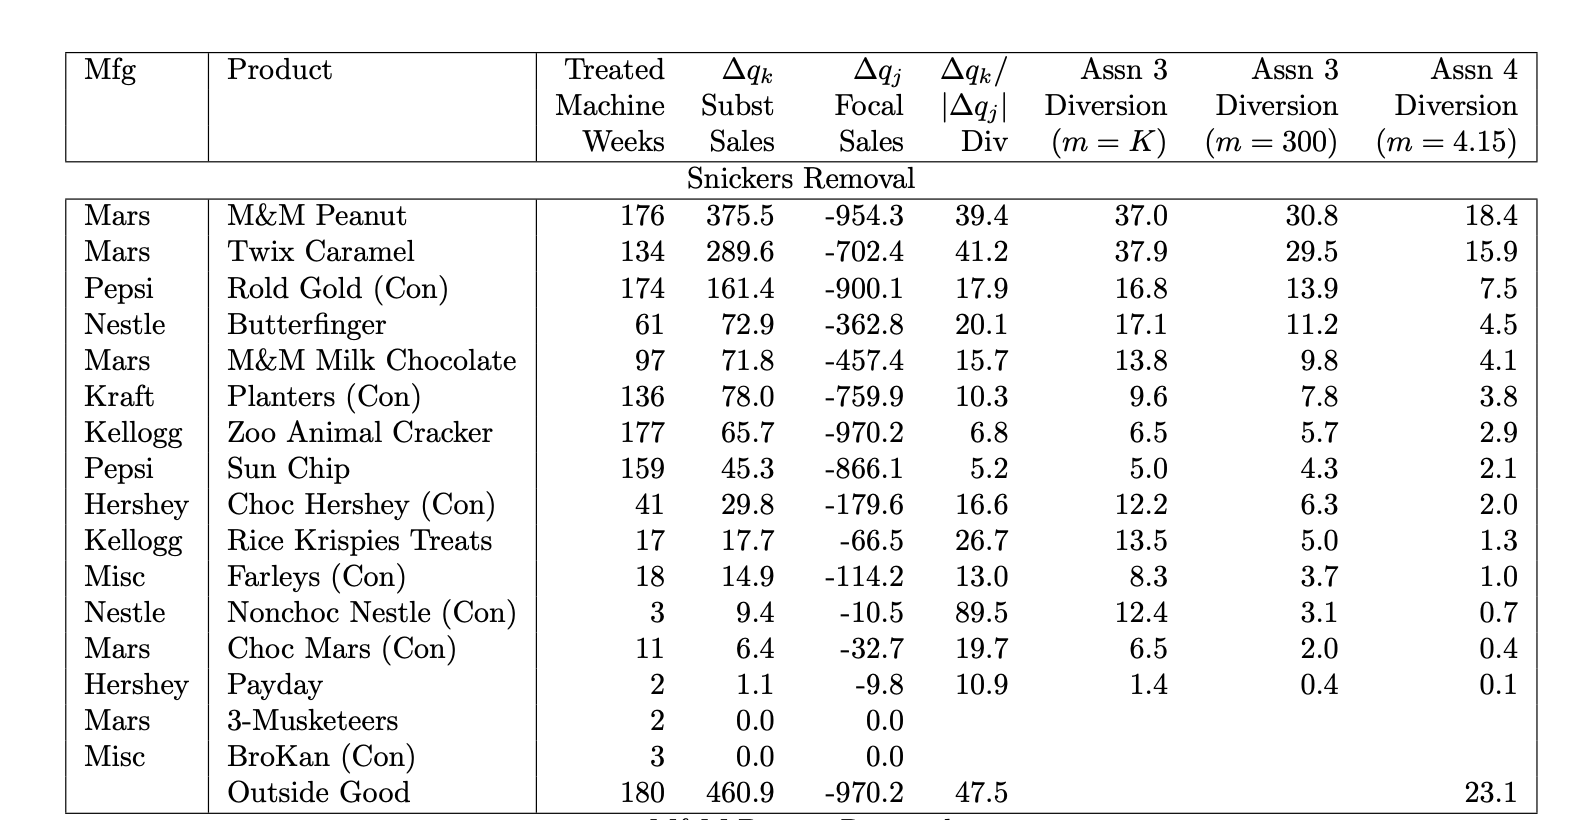
\includegraphics[height=0.8\textheight]{./resources/diversion.png}
\end{center}
\end{frame}

\begin{frame}{Fully Hierarchical Models: What's the point}
Suppose we want to estimate a lognormal distribution for income in different places
\begin{itemize}
\item Fully Pooled: estimate a single $(\mu,\sigma)$
\item Non-Pooled: estimate a separate $(\mu_k,\sigma_k)$ for each zip code
\item Paritally-Pooled: some combination of the two?
\begin{itemize}
\item Allow $\mu_k \sim F(\mu,\sigma)$.
\item estimate both the common (hyper) parameter and the group specific one.
\item Limit high variance from small groups.
\end{itemize}
\end{itemize}
\end{frame}


\begin{frame}{Fully Hierarchical Models}
Suppose we have several groups, each with their own mean:
\begin{align*}
b_{i} & \sim \mathcal{N}\left(0, \sigma_{b}^{2}\right) \\
\mu_{i} &=\mu+b_{i} \\
y_{i j} & \sim \mathcal{N}\left(\mu_{i}, \sigma_{y}^{2}\right)
\end{align*}
Or we could have written:
\begin{align*}
y_{i j}=\mu+\underbrace{b_{i}}_{\sim \mathcal{N}\left(0, \sigma_{b}^{2}\right)}+\underbrace{\epsilon_{i j}}_{\sim \mathcal{N}\left(0, \sigma_{y}^{2}\right)}
\end{align*}
That is there is a common mean $\mu$ and a group specific mean $b_i$.
\end{frame}

\begin{frame}{Fully Hierarchical Models}
\begin{align*}
y_{i j}=\mu+\underbrace{b_{i}}_{\sim \mathcal{N}\left(0, \sigma_{b}^{2}\right)}+\underbrace{\epsilon_{i j}}_{\sim \mathcal{N}\left(0, \sigma_{y}^{2}\right)}
\end{align*}
\begin{itemize}
\item Sometimes we interpret $b_i$ as a \alert{random effect}
\item In any case we will get some \alert{shrinkage} to the overall mean $\mu$
\item We could estimate by MLE if we know which $b_i$ corresponded to which $y_{ij}$ otherwise via Bayesian methods.
\end{itemize}
\end{frame}


\section*{Thanks!}




\end{document}
https://www.matteoparadisi.com/#Teaching